\subsection{Fonctionnement:}
Au sens large, un réseau intelligent associe l’infrastructure électrique aux technologies numériques qui analysent et transmettent l’information reçue. Ces technologies sont utilisées à tous les niveaux du réseau : production, transport, distribution et consommation.

\begin{itemize}[label=\textbullet]
\item \textbf{Un contrôle des flux en temps réel :} des capteurs installés sur l’ensemble du réseau indiquent instantanément les flux électriques et les niveaux de consommation. Les opérateurs du réseau peuvent alors réorienter les flux énergétiques en fonction de la demande et envoyer des signaux de prix aux particuliers pour adapter leur consommation (volontairement ou automatiquement).

\item \textbf{L’interopérabilité des réseaux :} l’ensemble du réseau électrique comprend le réseau de transport et le réseau de distribution. Le premier relie les sites de production d’électricité aux zones de consommation : ce sont les grands axes qui quadrillent le territoire. Le réseau de distribution s’apparente aux axes secondaires. Il achemine l’électricité jusqu’aux consommateurs finaux. Par l’échange instantané d’informations, les smart grids favorise une interopérabilité entre les gestionnaires du réseau de transport et ceux du réseau de distribution.

\item \textbf{L’intégration des énergies renouvelables au réseau :} les réseaux intelligents reposent sur un système d’information qui permet de prévoir à court et à long terme le niveau de production et de consommation. Les énergies renouvelables qui fonctionnent souvent par intermittence et de façon peu prévisible peuvent ainsi être mieux gérées.

\item \textbf{Une gestion plus responsable des consommations individuelle :} les compteurs communicants (ou compteurs évolués, « Linky » pour l'électricité) sont les premières versions d’application du réseau intelligent. Installés chez les consommateurs, ils fournissent des informations sur les prix, les heures de pointe de consommation, la qualité et le niveau de consommation d’électricité du foyer. Les consommateurs peuvent alors réguler eux-mêmes leur consommation au cours de la journée. De leur côté, les opérateurs du réseau peuvent détecter plus vite les pannes.
\end{itemize}

\begin{figure}[h]
	\centering
    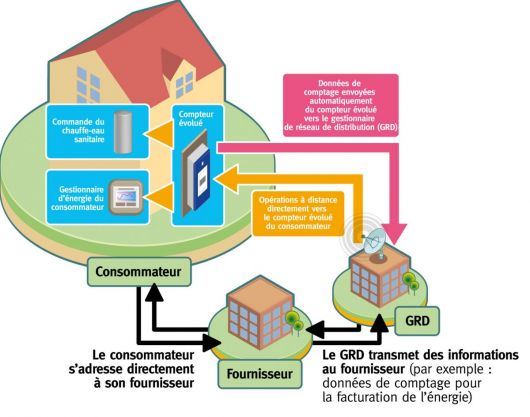
\includegraphics[scale=0.5]{img/part2/1.2}
    \caption{Fonctionnement du Smart Grid}
\end{figure}